\pagestyle{headings}
\chapter{GEMC geometry}
Geometry created with \textit{Coatjava} can be translated to \textit{GEMC} readable format in order to use exactly the same geometry for reconstruction and simulations.

We will first discuss how to generate active detectors geometry using the same \textit{Coatjava} classes. For this, we use \textit{groovy} code that generates text files defining the geometry, materials, banks and hits for each detector.

Then we describe the procedure used to generate inactive materials for \textit{GEMC}.

\section{AHDC}
The link between \textit{Coatjava} and \textit{GEMC} is \textcolor{magenta}{\texttt{factory\_ahdc.groovy}} code. Inside, we call \\ 
\texttt{MYFactory\_ALERTDCWire factory = new MYFactory\_ALERTDCWire();} \\ 
We get all the volumes using \\
\texttt{Component comp = } \\ \texttt{ahdc.getSector(isec).getSuperlayer(isl).getLayer(ilay).getComponent(icomp);}

and we get the $(X,Y)$ of all the smallest volumes - trapezoides! \textcolor{magenta}{Reminder: AHDC cell is not a simple trapezoide, but a union of 2 trapezoides!} To generate the real AHDC cell, we arrange the trapezoides in pairs, giving them the same identifier\footnote{An identifier is just a number given to a volume. When an interaction happens in 2 different volumes($\neq identifier$) then different hits are recorded. In AHDC, we do not distinguish between the 2 sub-cells of the same cell, thus they have the same identifier.}. Thus, one AHDC cell is made of 2 sub-cells.

For example, for one AHDC cell we have different sub-cell names and the same identifier:

\texttt{superlayer0\_layer0\_ahdccell26\_subcell1 ... G4GenericTrap ... 0 0 26}\\
\texttt{superlayer0\_layer0\_ahdccell26\_subcell2 ... G4GenericTrap ... 0 0 26}

where identifier $= 0 \ 0 \ 26$.

Text file \textcolor{blue}{\texttt{ahdc\_\_volumes\_default.txt}} lists all the volumes, their shape, position, coordinates of the vertices, names and identifiers and it is generated by \texttt{factory\_ahdc.groovy} code. Text file \textcolor{blue}{\texttt{ahdc\_\_parameters\_default.txt}} gives the number of components in each superlayer and layer and it is also generated by \texttt{factory\_ahdc.groovy} code. 

Next step is to associate a mother volume, a material, a sensitivity, and a hit type to each active volume. This association is given by \texttt{geometry\_java.pl} perl code. In addition, it is necessary to have:
\begin{itemize}
	\item \texttt{materials.pl}, where the needed materials are defined by their compositions;
	\item \texttt{bank.pl}, where the outputs that we want into digitization are defined. Each detector has its own bank number. AHDC bank  number is 2300, \texttt{define\_ahdc\_bank("ahdc", 2300)}.
	\item \texttt{hit.pl}, where hit name and characteristics are defined. For AHDC, hit name is "ahdc".
\end{itemize}

Finally, \textcolor{brown}{\texttt{ahdc.pl}} code calls all the mentioned above parts and generates text files that can be given to \textit{GEMC} in order to run a simulation. These last text files are:
\begin{itemize}
	\item \texttt{ahdc\_\_geometry\_default.txt}, list of all the active volumes with correspondant material and sensitivity.
	\item \texttt{ahdc\_\_bank.txt}, \texttt{ahdc\_\_hit\_default.txt}, \texttt{ahdc\_\_materials\_default.txt}.
\end{itemize}
  
\begin{figure}[H]
	\centering
	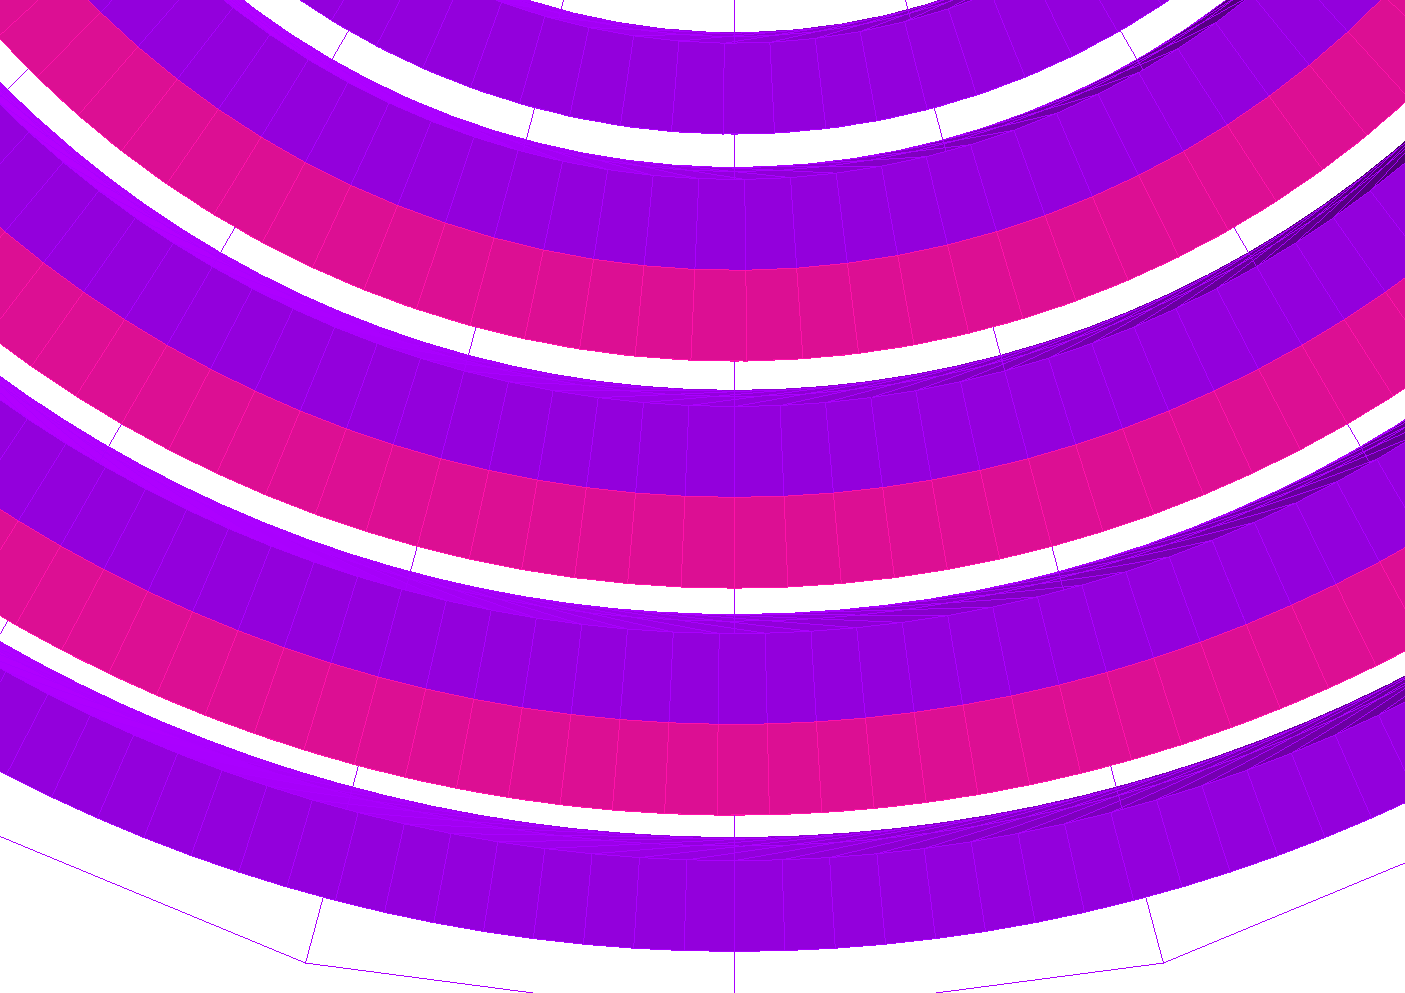
\includegraphics[width=0.7\textwidth]{gemc_ahdc_face_detail1.png}
	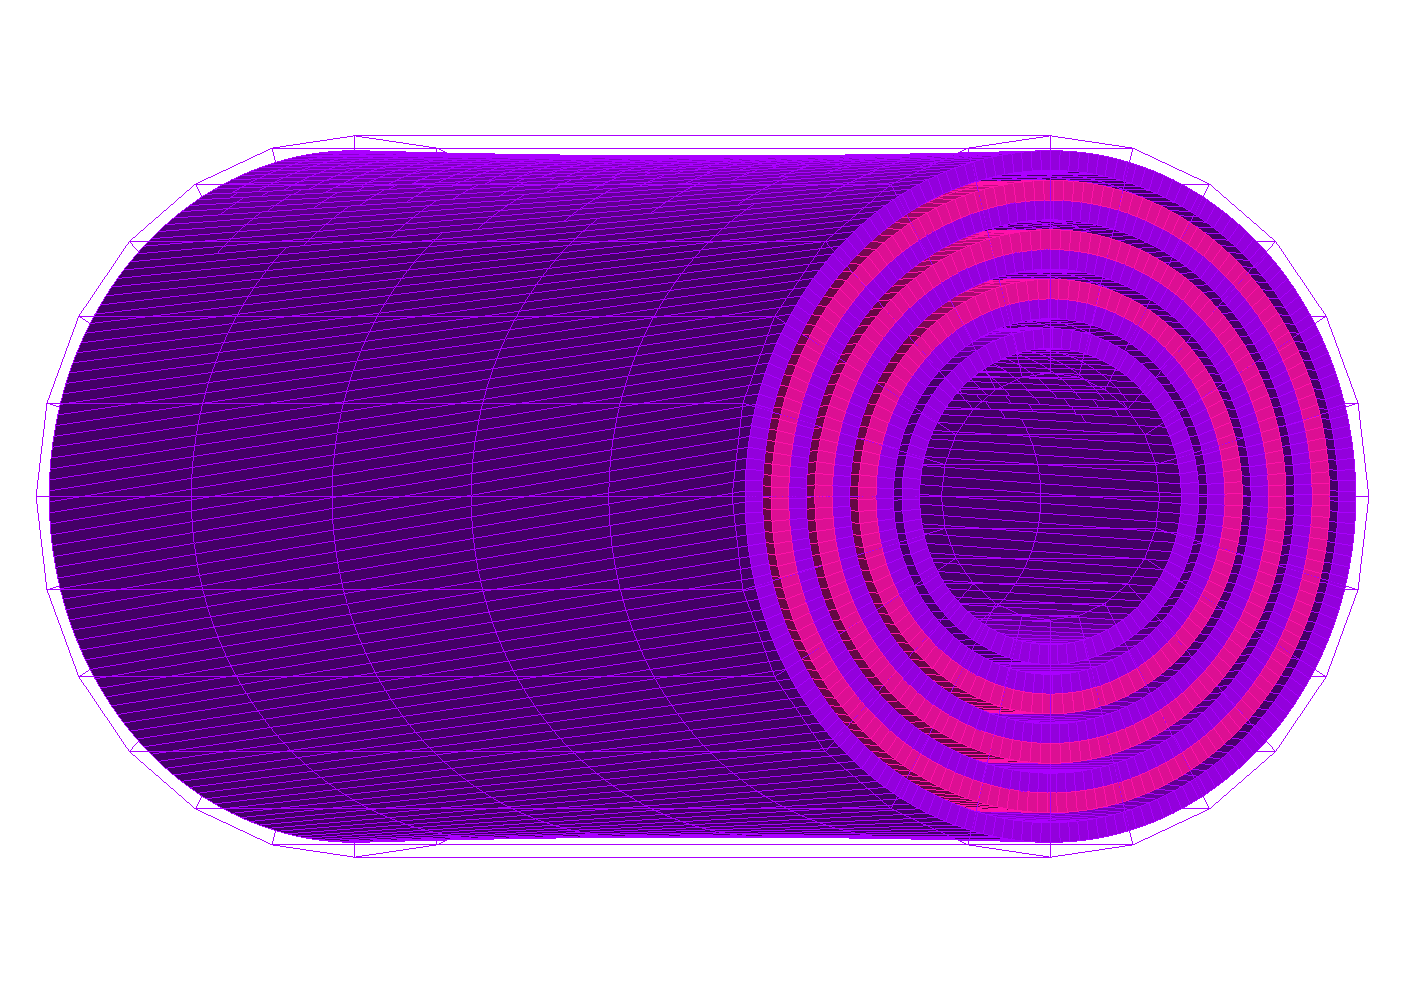
\includegraphics[width=0.7\textwidth]{gemc_ahdc_profile.png}
	\caption{AHDC geometry in \textit{GEMC}. Mother volume is visible.}
	\label{fig:ahdc_gemc}
\end{figure}


\newpage
\section{ATOF}
The same procedure as above has to be applied to generate ATOF geometry for \textit{GEMC}. 

The link between \textit{Coatjava} and \textit{GEMC} is \textcolor{magenta}{\texttt{factory\_atof.groovy}} code. Inside, we call \\ 
\texttt{MYFactory\_ATOF\_NewV2 factory = new MYFactory\_ATOF\_NewV2();} \\ 
We get all the volumes using \\
\texttt{Component comp = atof.getSector(isec).getSuperlayer(isl).getLayer(ilay).getComponent(icomp);}

We get the $(X,Y)$ of all the trapezoides. For ATOF, one trapezoide = one active cell. We give the names and identifiers for each volume. For example:

\texttt{sector1\_superlayer1\_layer6\_paddle5 ... G4GenericTrap ... 1 1 6 5} \\
\texttt{sector1\_superlayer1\_layer6\_paddle6 ... G4GenericTrap ... 1 1 6 6}

where identifiers are $1 \ 1 \ 6 \ 5$ and $1 \ 1 \ 6 \ 6$.

We obtain the text files \textcolor{blue}{\texttt{myatof\_\_volumes\_default.txt}} and \textcolor{blue}{\texttt{myatof\_\_parameters\_default.txt}}. 

Next, we give the text files and {\texttt{geometry\_java.pl, \ materials.pl, \ bank.pl, \ hit.pl} , corresponding to ATOF, to the \textcolor{brown}{\texttt{atof.pl}} code. Finally, we obtain the last text files:
\begin{itemize}
	\item \texttt{myatof\_\_geometry\_default.txt}, list of all the active volumes with correspondant material and sensitivity.
	\item \texttt{myatof\_\_bank.txt}, \texttt{myatof\_\_hit\_default.txt}, \texttt{myatof\_\_materials\_default.txt}.
\end{itemize}

For ATOF the bank number is 2200. ATOF hit name is "myatof". 

\begin{figure}[H]
	\centering
	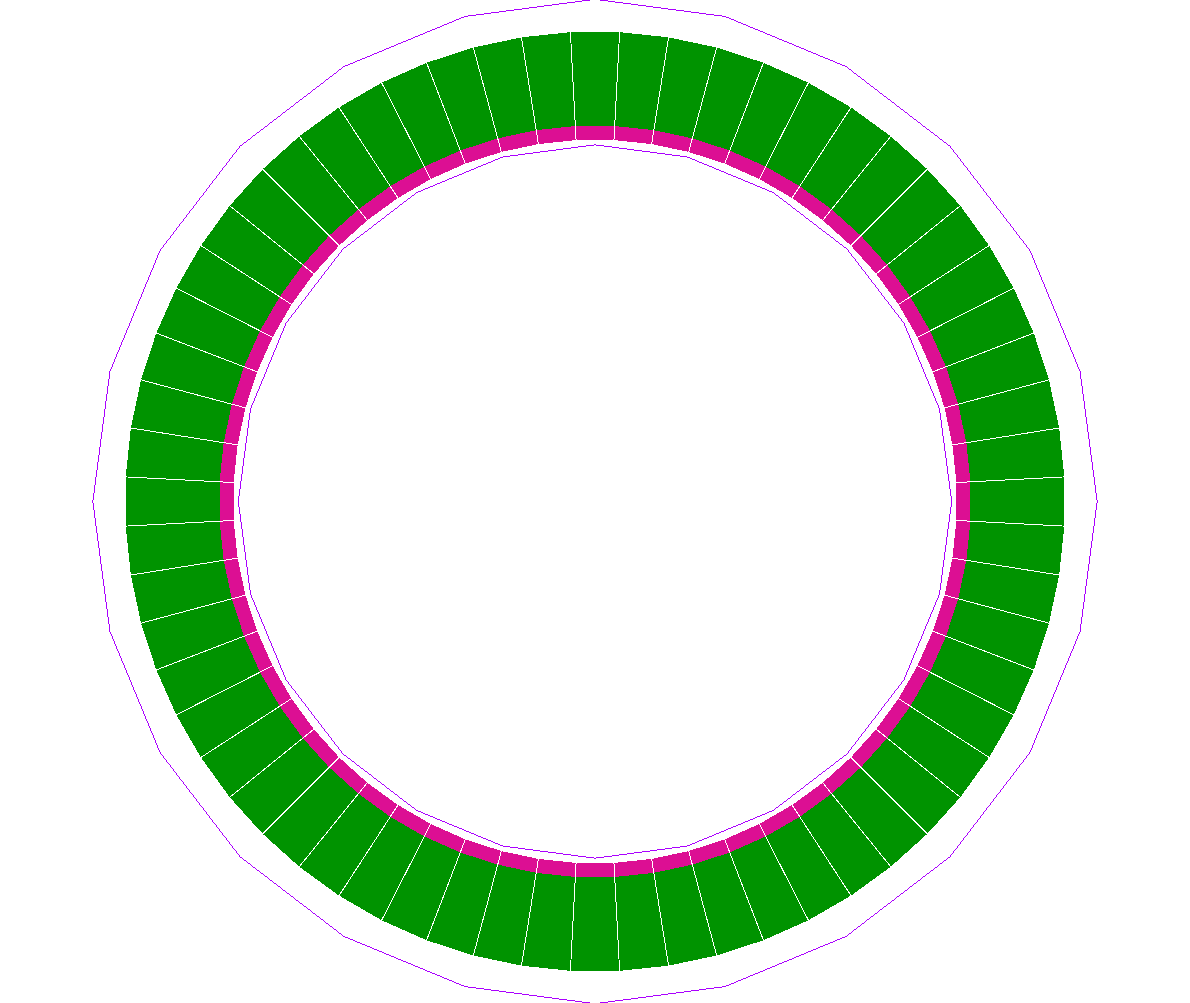
\includegraphics[width=0.8\textwidth]{gemc_atof_face.png}
	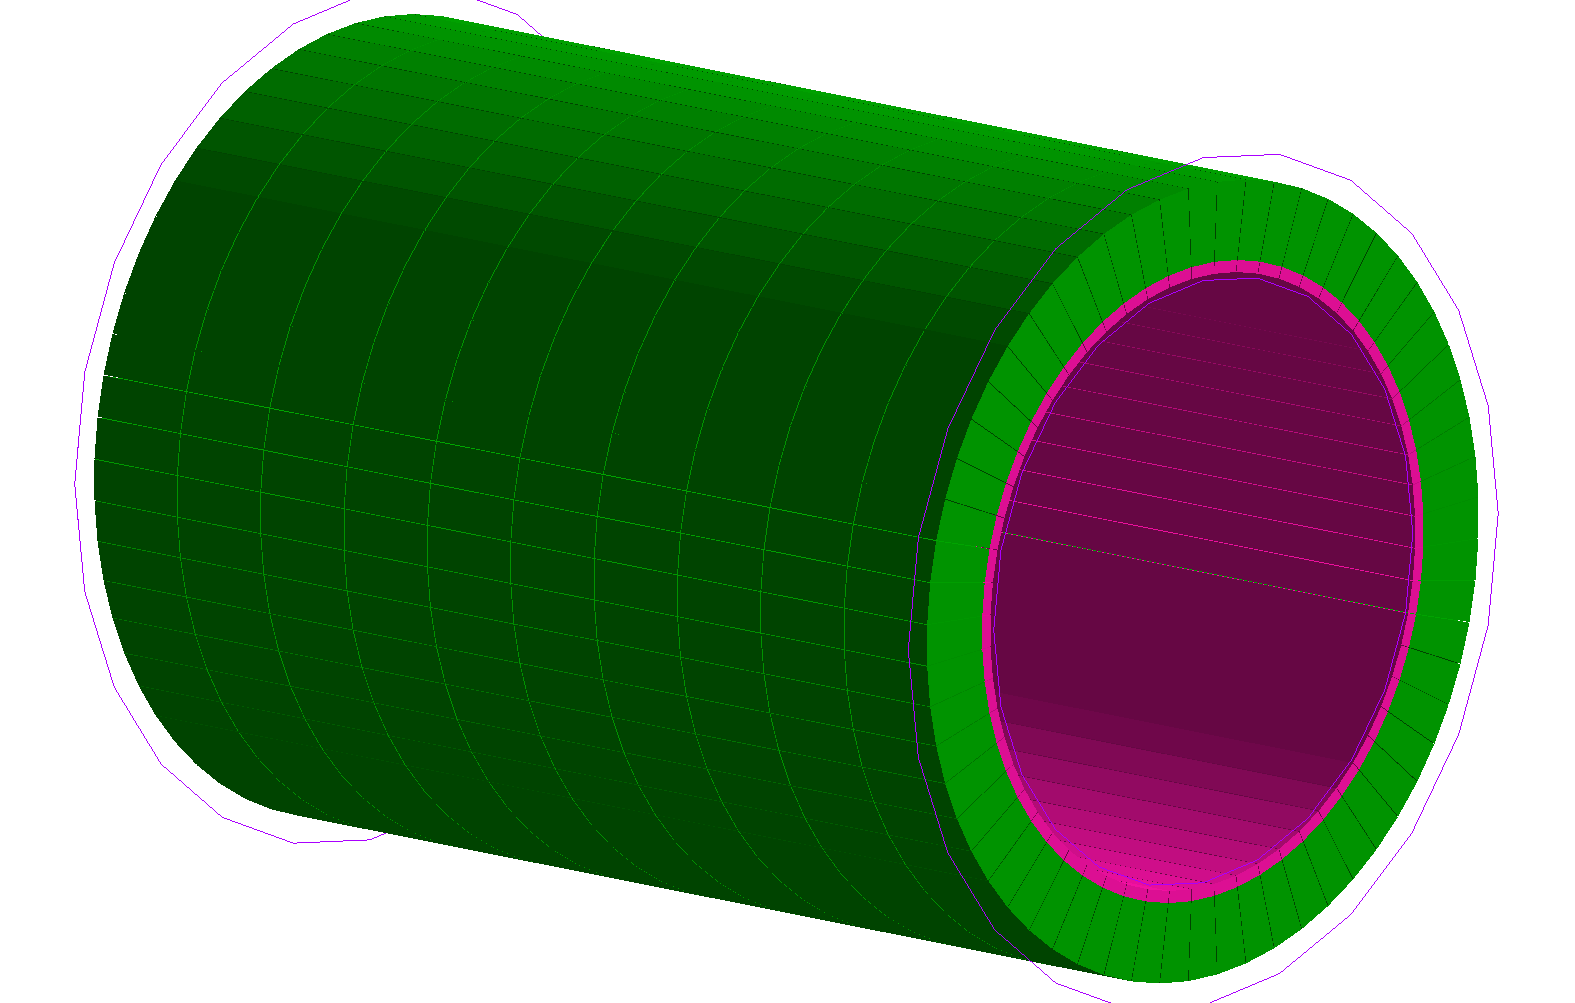
\includegraphics[width=0.8\textwidth]{gemc_atof_profile.png}
	\caption{ATOF geometry in \textit{GEMC}. Mother volume is visible.}
	\label{fig:atof_gemc}
\end{figure}



\newpage	
\section{Non active geometry}
This section describes the geometry structures that are not active and not used into reconstruction. Nevertheless, they have to be taken into account due to the materials stopping power. These geometries do not have \textit{Coatjava} equivalent and they are generated directly by perl codes.
	
	\subsection{ALERT target}
	The ALERT target is generated from \texttt{gemc/detectors/clas12/targets/...}. The geometry ( = a straw) is defined in \texttt{geometry.pl} with variation $ = "alert"$. Target is filled with $5$ atm deuterium gas. The straw is 300 mm long, wall is made of $G4\_Kapton$ and $0.060$ mm thick. Upstream and downstream windows are in $G4\_Al$ and $0.030$ mm thick. Inside radius of the target is $3$ mm. Materials are defined in \texttt{ materials.pl}. The text files that can be given as \textit{GEMC} inputs are: \texttt{target\_\_geometry\_alert.txt} and \texttt{target\_\_materials\_alert.txt}.
	\begin{figure}[H]
	\centering
	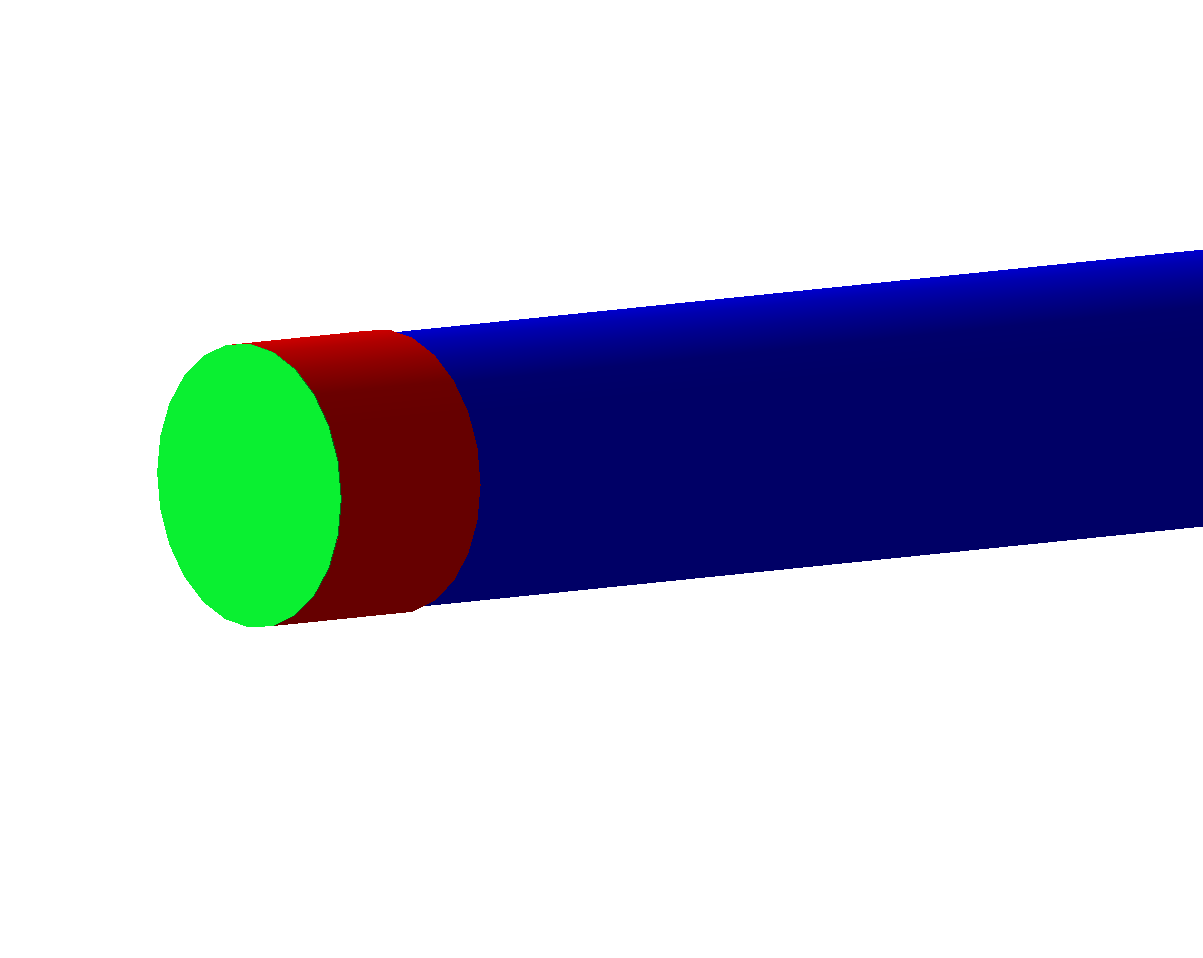
\includegraphics[width=0.4\textwidth]{gemc_ALERT_TG_upstreamEnd2.png}
	\caption{ALERT target upstream end detail.}
	\label{fig:tg_gemc}
	\end{figure}	
	
	\subsection{Helium bag}
	The Helium bag is a cylinder placed between the target and the beamline pipe. This volume replaces the \texttt{"detector name = airPipe"} volume, that has to be indicated explicitely in the gcard that will be used for the simulation. Geometry is described in \texttt{geometry.pl}. Outter radius is $\approx 25$ mm  and the length $300$ mm. Downstream window is plane disc. Upstream window has an inner radius of $3.1561$ mm. The bag is made of $G4\_Al$ and filled with $G4\_He$ (1 atm.).		
	\begin{figure}[H]
	\centering
	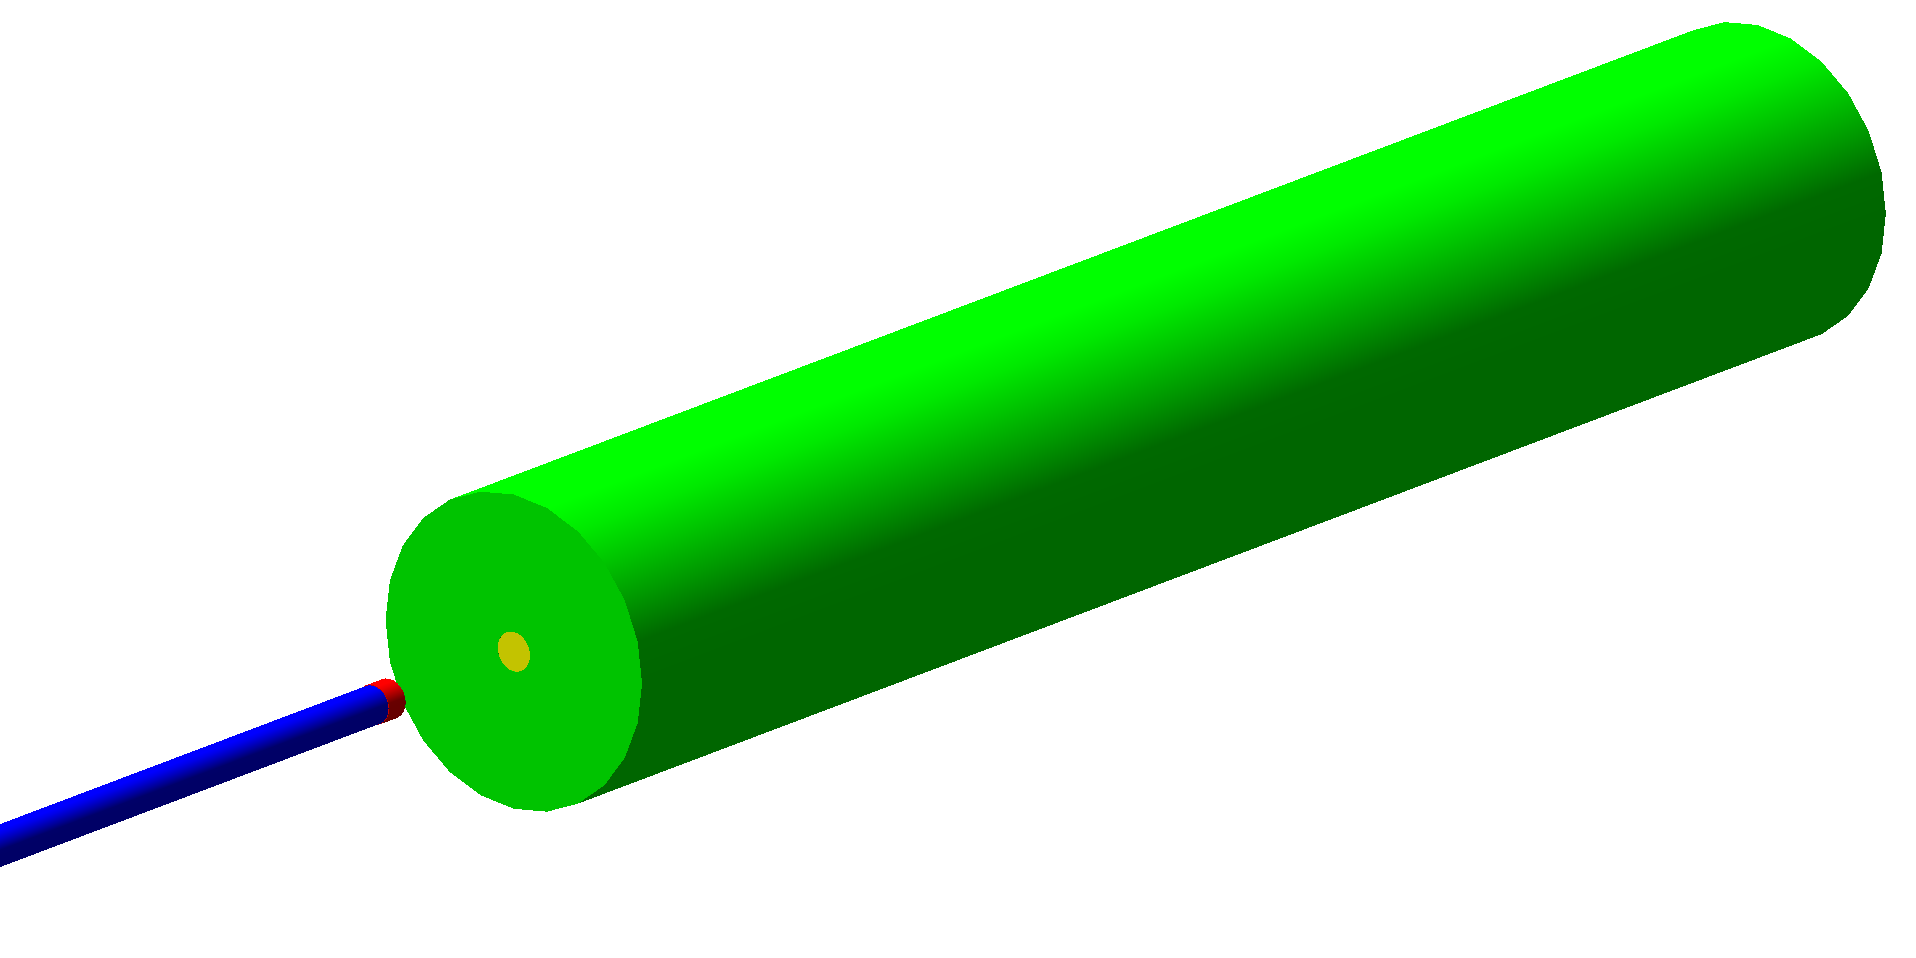
\includegraphics[width=0.6\textwidth]{gemc_ALERT_TG_andHebag_zoom.png}
	\caption{ALERT He bag and target.}
	\label{fig:hebag_gemc}
	\end{figure}	
	
\subsection{External support structure}
	The complex geometry of ATOF mechanics and the 15 ribs is simplified to layers of  concentrical cylinders that surround ATOF + AHDC + target setup. The back (= upstream) and front (= downstream) plates are plane discs. Front plate consists of Macor, carbon and copper consecutive discs. The geometry is defined into \texttt{alertshell.pl} code. For non active geometry the assignement of identifiers, sensitivity and hit type is not necessary. The \texttt{materials.pl} description is mandatory. \\
	The use of  \texttt{> /.alertshell.pl config.dat} generates text files that have to be given as \textit{GEMC} input: \texttt{alertshell\_\_geometry\_original.txt, alertshell\_\_materials\_original.txt}.
	\begin{figure}[H]
	\centering
	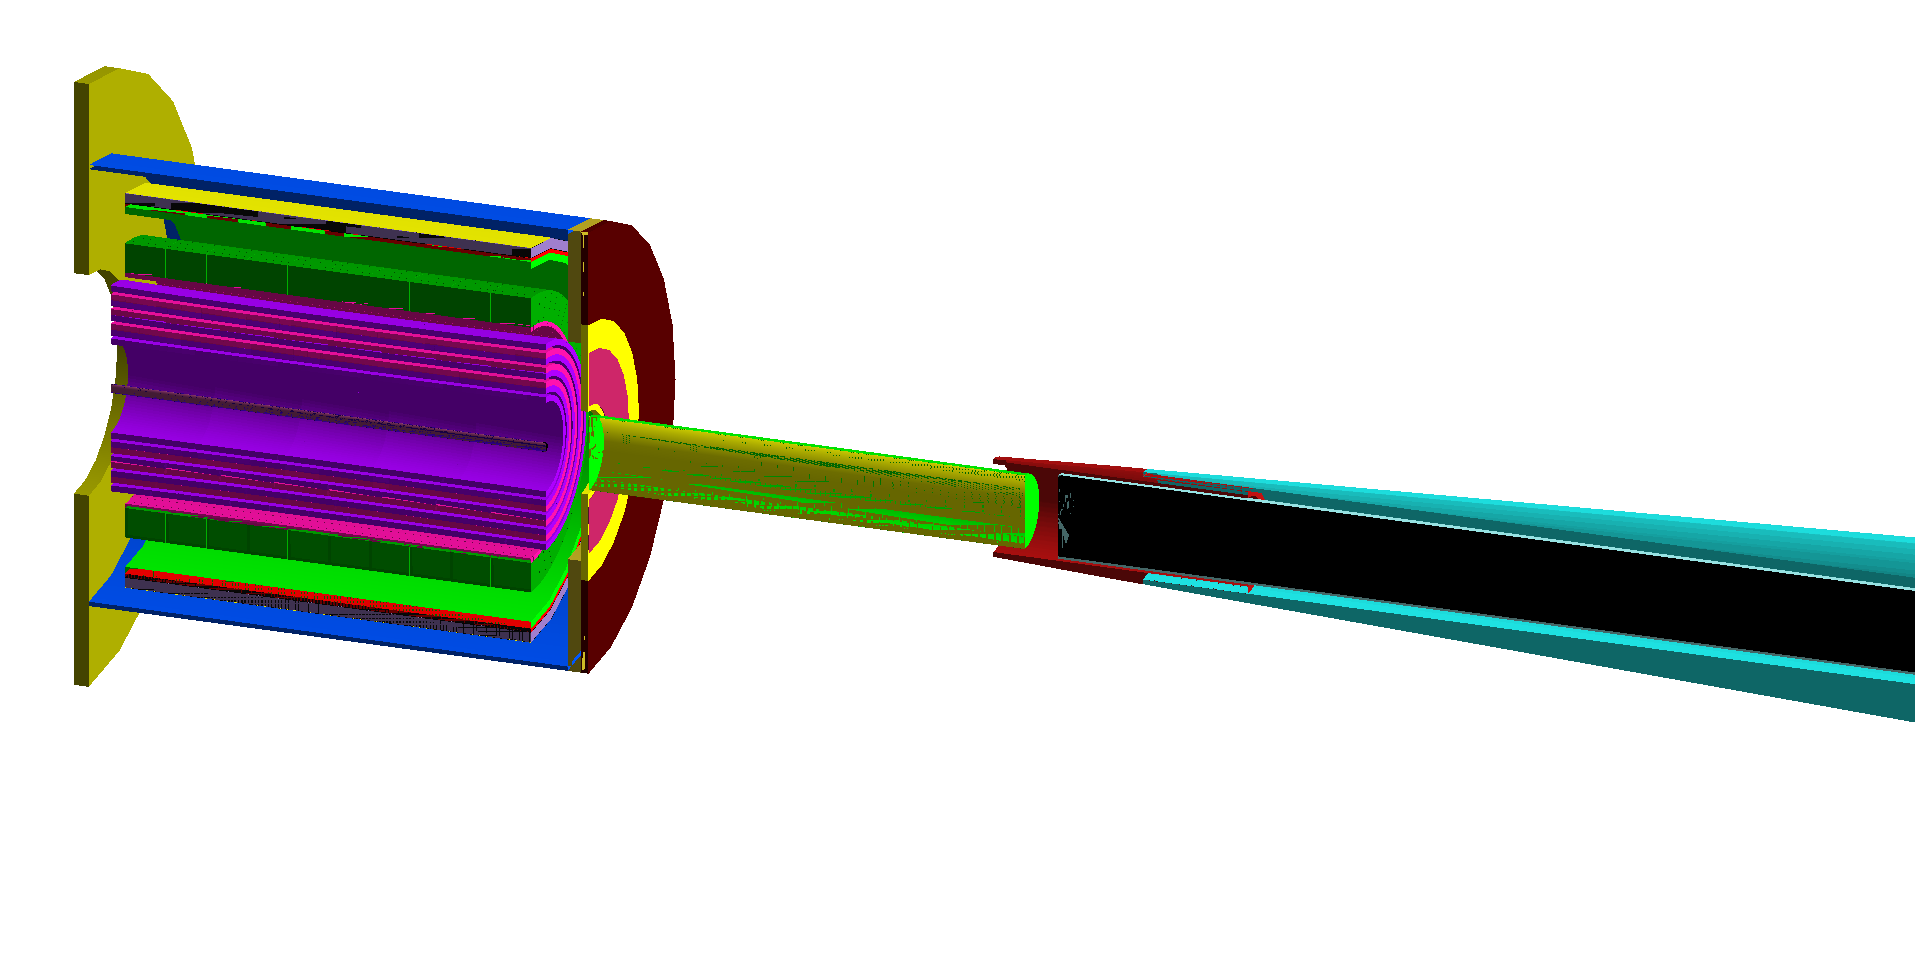
\includegraphics[width=0.6\textwidth]{gemc_HeBag_ALERT_cut_1.png}
	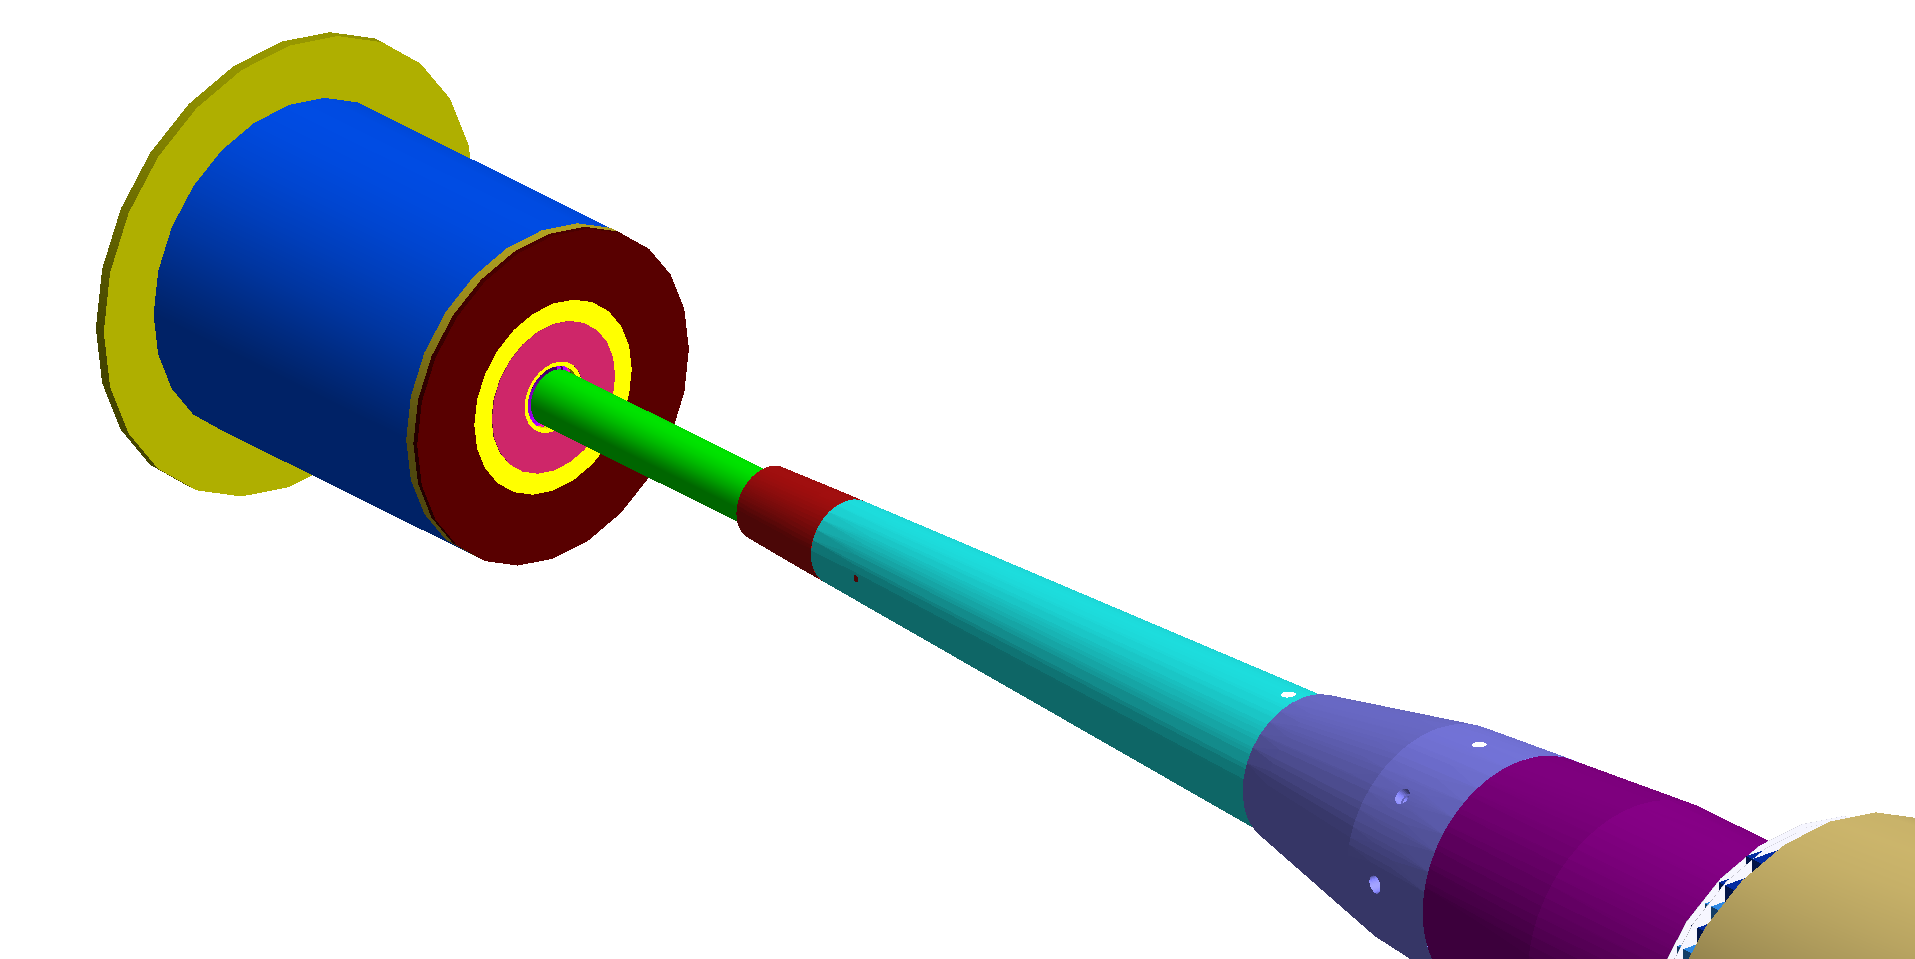
\includegraphics[width=0.6\textwidth]{gemc_HeBag_ALERT_2.png}
	\caption{External shell surrounding (AHDC + ATOF + target) \& He bag in green.}
	\label{fig:hebag_gemc}
	\end{figure}
	
	
\begin{comment}		
Figures \ref{fig:setup_gemc}, \ref{fig:setup1_gemc} show the global ALERT setup and the addition of some CLAS12 detectors.
\begin{figure}[H]
	\centering
	%\includegraphics[width=0.8\textwidth]{}
	%\includegraphics[width=0.8\textwidth]{}
	\caption{...}
	\label{fig:setup_gemc}
\end{figure}

\begin{figure}[H]
	\centering
	%\includegraphics[width=0.8\textwidth]{}
	%\includegraphics[width=0.8\textwidth]{}
	\caption{...}
	\label{fig:setup1_gemc}
\end{figure}
\end{comment}